\chapter{Future Directions}
It has been such a blessing to work with so many talented colleagues and collaborators; the problem is that there are too many good ideas and not enough time. For this reason, I would like to highlight a few exciting directions I was unable to pursue and, hopefully, they will spark even better ideas in those that follow.

\section{The Multi-Step Invasion Assay}
\paragraph{Note:}Individuals leading the development of this idea include Ben Casavant, Lauren Bischel, Edmond Young, and Erwin Berthier.

The multi-step invasion assay is a concept that is currently taking hold, bringing together multiple technologies and individuals in the laboratory with an exciting potential to enable new studies and insights that have been previously unavailable. The assay focuses on the process of metastasis, which involves multiple steps including intravasation, attachment, extravasation, invasion. Fig \ref{Chap:FutureDirections:fig:multiStep} illustrates the concept of the multi-step assay and how various components relate to different events during metastasis.

\begin{figure}[!ht]
\centering
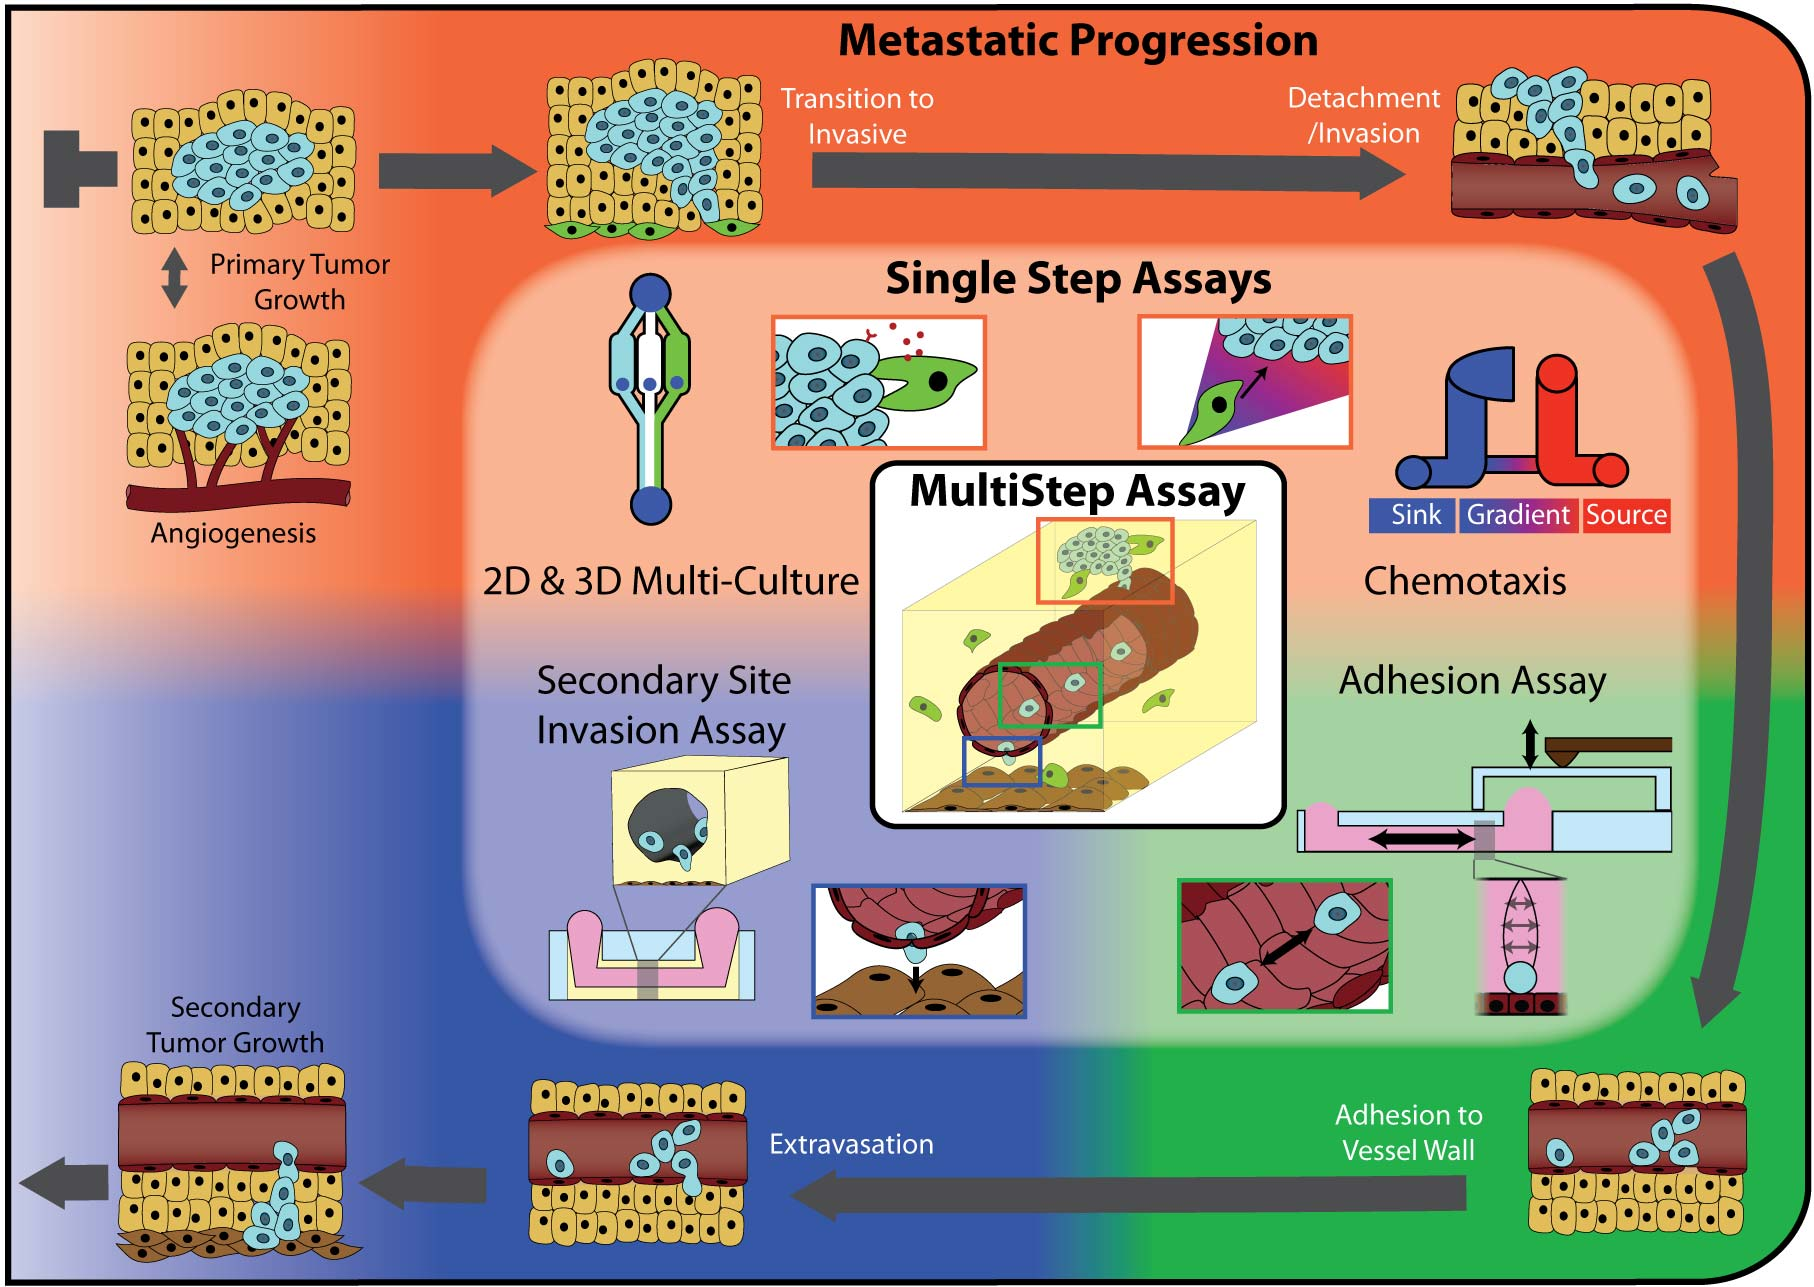
\includegraphics[width=5in]{MultiStep.jpg}
\caption{\textbf{The multi-step assay}. This figure was created by Ben Casavant and Lauren Bischel with contributions from other involved.}
\label{Chap:FutureDirections:fig:multiStep}
\end{figure}

The assay incorporates the ability to form a lumen in a 3-D matrix coated with endothelium within a mirochannel containing tumor and\slash or stromal cells. Tumor cells can be introduced under oscillatory flow to mimic the environment in which tumor cell attachment and extravasation occurs. The influence of tumor cells, stromal cells, and drug therapies can be introduced or removed to examine how each influence each of these metastatic events. It also offers a unique model in which to study the role of the endothelium and how each of the components influences that role.

The ability to study these events in a single device would be a unique contribution to the study of metastasis. In addition, we also have tools and expertise to examine each event individually using `single-step' assays. The modularity of the single-step assays also facilitates various combinations of subsets of the microenvironmental components included in the multi-step assay.

\section{BeadSpot Assay for Targeted Detection of Cell Secretions}

\paragraph{Note:}This concept was been developed in equal collaboration with Scott Berry and Lindsey Maccoux.

Cell secretions are of interest as a functional readout that is well suited for studying rare-cell populations such as circulating tumor cells. Cell secretions are typically measured for entire populations using techniques such the ELISA instead of for individual cells. However, given our interest in learning more about the heterogeneity of circulating tumor cells, a single cell readout would provide a much more relevant readout. Single-cell readouts of cell secretions are typically done using an EpiSpot or FluoroSpot which capture secreted proteins using antibodies adsorbed to a porous membrane. The captured proteins form a spot on the membrane around secreting cells which can be detected after staining using a microscope.

We hope to increase the specificity and sensitivity of these Spot-based assays through the use of beads. The beads are functionalized with two antibodies, one specific to the cell type of interest and the other specific to the secretion of interest. The goal is to bind the beads to a target cell population and capture secretions as they leave the cell, increasing both specificity and sensitivity relative to membrane based methods. 

Fig \ref{Chap:FutureDirections:fig:beadSpot} illustrates the results of preliminary work developing this method. Results are as expected. The beads bound cells that express EpCAM (LNCaP and MCF-7) while only detecting PSA from PSA secreting cells (LNCaP). Future work is expected to include the use of fluorescent beads to help quantify secretion levels by normalizing detection levels for each cell by the number of beads attached to the cell.

\begin{figure}[!ht]
\centering
\includegraphics[width=5in]{BeadSpot.pdf}
\caption{\textbf{BeadSpot assay for targeted detection of secretions from individual cells}. Each image indicates the cell-type and the types of antibodies that exist on the detection beads. Image provided by Scott Berry.}
\label{Chap:FutureDirections:fig:beadSpot}
\end{figure}

The use of beads allows us to detect secretion on surfaces other than porous membranes which are not always conducive to cell culture or cell attachment. It also allows the preparation of the beads in batches, increasing repeatability between assays as opposed to porous membranes which must be prepared separately each time. Although this method can be used with microscale culture technology, it is not limited to microscale use and could help to provide a unique readout for challenging rare-cell applications.

\section{3-D Invasion Assays}
\paragraph{Note:} Invasion of tumor cells is an important topic in our laboratory and thus many of us are interested in different ways to study this process. Recently, it has become apparent the many of us (\eg, Eric Sackmann, Erwin Berthier, Ben Casavant, Lauren Bischel, Edmond Young, and myself) are approaching this problem in parallel, albeit for slightly different reasons, and may be able to take advantage of each others findings. Some of this information is summarized here along with a recent advance that could bring a microscale invasion assay closer to a reality.

At the heart of an invasion assay is the need to seed cells on a 3-D matrix that can support invasion. It would also be beneficial if a second cell type could be introduced into that matrix. Lauren has shown the ability to produce lumens in microchannels enabling high-throughput production of a biologically relevant structure for studying epithelial structures and is amenable to invasion. Together, Lauren and Ben have shown the ability to use the lumen to study invasion but have arrived at a critical conclusion; enabling a readout of invasion can be more difficult than developing a method to perform invasion. For example, it could be difficult to use confocal imaging to quantify invasion in an array of channels. Thus, one advantage of the transwell that should be recognized is the readout. If a cell migrates through the membrane of a transwell, the cell falls into the bottom compartment, thus allowing invasion to be quantified by simply counting the number of cells that have made it to the bottom compartment. Thus, it may not be the relevance of the assay that drives its use, but the ease of the readout. I believe this is an important piece of information they have come to realize and is important for others in this area to keep in mind. 

I would also like to highlight a method developed in previous work by Eric Sackmann and Erwin Berthier in which they are able to coat just the bottom of a channel with a 3-D matrix. This capability could be very important in future embodiments of invasion assays as it allows for easy seeding of cells on top of the matrix and facilitates replenishment of media.

My interest in the invasion stemmed from interest in the multi-step assay where I had hoped to perform adhesion assays on an endothelium where the endothelium is separated from a layer of stromal cells using a 3-D matrix. The method developed by Erwin and Eric was very intriguing for this purpose but had one major drawback for my application. In their approach it is difficult to control the curvature of the gel surface in the bottom of the channel. Given that channel height significantly affects the shear in a channel, variability in the channel is difficult to accommodate. The curvature is variable because it is difficult to control the volume of dispensed gel with enough accuracy to fill the channel bottom repeatably. This was also a concern of Eric's and in joint conversation about this with Edmond, we ventured to solve this issue using another passive solution. A large reservoir port connected to the gel upon loading of the channel bottom can be used as a means to control curvature. By using a large reservoir port, the curvature does not change significantly with volume providing a more repeatable gel coating. Initial tests have found this approach to work and could be used to significantly improve the flatness of the gel coating.

In summary, many of the pieces are falling into place for some interesting advances in the area of invasion assays. Although each of us might be using this type of device for very different reasons, there are common issues that we face that are worth recognizing and addressing together that could result in a new approach that could have a broad impact across many different areas of biology, as illustrated by the interest and efforts of so many in our own lab.



